\chapter{Custom Models}

\setcounter{figure}{0}
\setcounter{table}{0}

\label{sec:CustomModels}

\section{Introduction to Custom Models}
\label{sec:IntroductiontoCustomModels}

Custom models are part of the advanced features available in OptimumTire. This fucntionality gives users the flexibility to include user developed custom models within the OptimumTire environment. With the custom models feature users can write their own models in house, therefore keeping proprietary models confidential and providing the ability to tailor models to the exact specifications required. Custom models need only to be coded once, they can then be used repeatedly and as efficiently as any of the hard coded models available within OptimumTire.
The custom model package is an advanced feature which requires an additional activation license available by contacting ~\href{mailto: engineering@optimumg.com}{engineering@optimumg.com}\\

\section{Creating Custom Models}
\label{sec:CreatingCustomModels}
Custom models are based on a template written in C\# this template is provided by OptimumG with the purchase of the custom models package. To create a new model the user must first define a .dll (dynamically linked library) file which can then be loaded into OptimumTire. This file references the template provided by OptimumG so it must follow a certain syntax that makes it compatible with OptimumTire. This syntax is outlined in Sections~\ref{sec:CreatingaCoefficientFile} and ~\ref{sec:CreatingaCalculationFile}. The user .dll contains a list of coefficients and equations that define the user's custom model.

An example project is included with OptimumTire to provide an example that users can copy and edit when developing custom models. The project is installed in My Documents on the users machine and can be opened with Visual C\#.

\subsection{Software Requirements}
\label{sec:CustomModelsSoftwareRequirements}

The custom model template is written in Visual C\# a CLI (Common Language Infrastructure) language. In order to create a custom model the user must first download a version of Visual C\# by Microsoft. This software is available as a free \textsl{Express Edition} for the general user or \textsl{Visual Studio Professional Edition} for professional software developers. For the purposes of creating OptimumTire custom models the \textsl{Visual C\# Express Edition} is sufficient. The download is availble at the following site ~\href{http://www.microsoft.com/express/Downloads/#2010-Visual-CS}{www.microsoft.com/express/Downloads}

OptimumTire requires two files a \textsl{Coefficient File} and a \textsl{Calculation File} to define a model. The follwing sections outline how to create these files.

\subsection{Creating the Custom Model Project}
The first step in creating custom model is to create a new C\# project with the coefficient and calculation classes. To do this open Visual Studio or Visual C\#. Create a new model from the file menu, select \textsl{C\# Class Library} and enter the name of your model as shown.

 \begin{figure}[H]
	\centering
		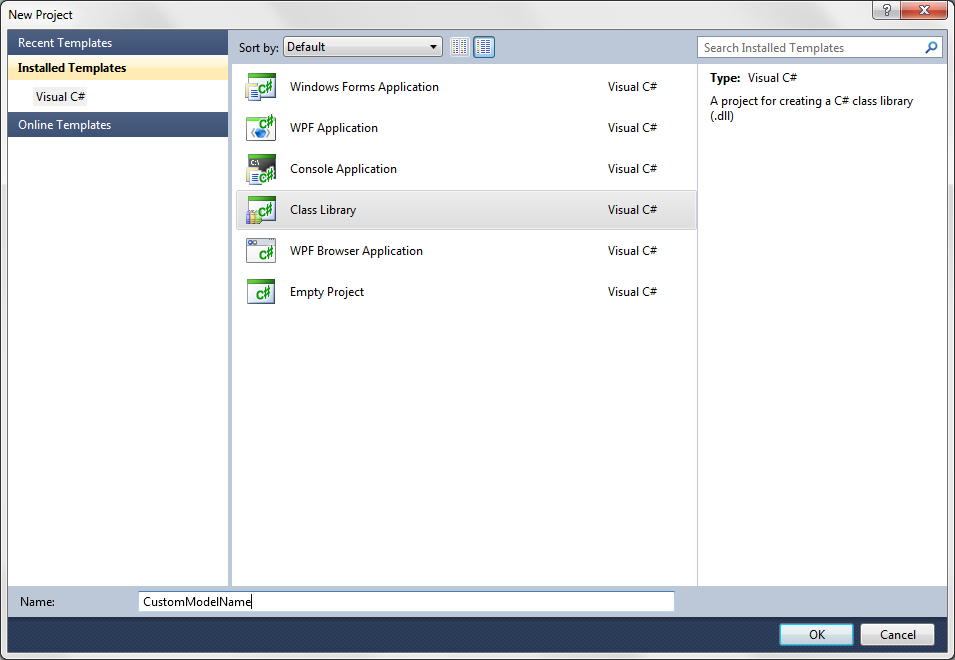
\includegraphics[width=1.0\textwidth]{NewCustomModelProject.png}
	\caption{Creating a New Project}
	\label{fig:CreatingaNewProject}
\end{figure}

Alternatively you can open the example project provided with OptimumTire, modify it and save it under a different name.

Next right click on the project just created and select add->new item to add a class to the project.

 \begin{figure}[H]
	\centering
		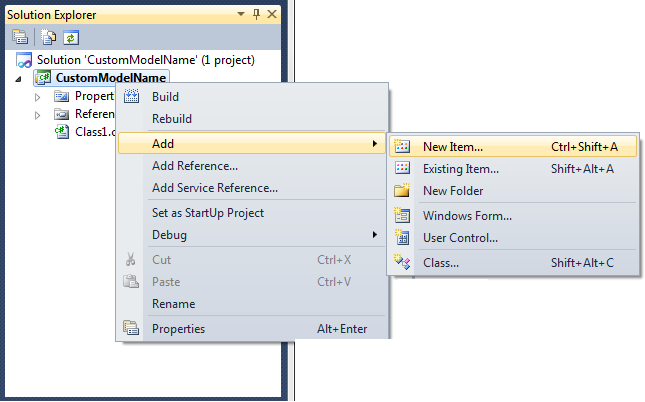
\includegraphics[width=1.0\textwidth]{NewCustomModelClass.png}
	\caption{Creating a New Class}
	\label{fig:CreatingaNewClass}
\end{figure}

Add two classes, the coefficient class and the calculation class. Name these classes \textsl{CustomTireModelCoef} and \textsl{CustomTireModelCalculation}. Save the project and then continue with the following steps.

\subsection{Referencing the Custom Model Template}
\label{sec:ReferencingtheCustomModelTemplate}

Once the project has been created the next step is to add the reference for the custom model template. Without this reference the custom model classes defined by the user cannot inherit from the template.
To add a reference to a project first right click on the C\# project and select add reference from the dropdown menu as shown in Figure~\ref{fig:CreatingaReference}.

 \begin{figure}[H]
	\centering
		\includegraphics[height=0.3\textheight]{creatingReference.png}
	\caption{Creating a Reference}
	\label{fig:CreatingaReference}
\end{figure}

Select the browse tab in the add reference dialog and browse to the OptimumTire installation folder. Select the CustomTireModelTemplate.dll and select OK as shown in Figure~\ref{fig:SelectingtheReferencedll}. The reference to the template.dll should now appear in the project references folder in the Visual Studio Solution Explorer. 

 \begin{figure}[H]
	\centering
		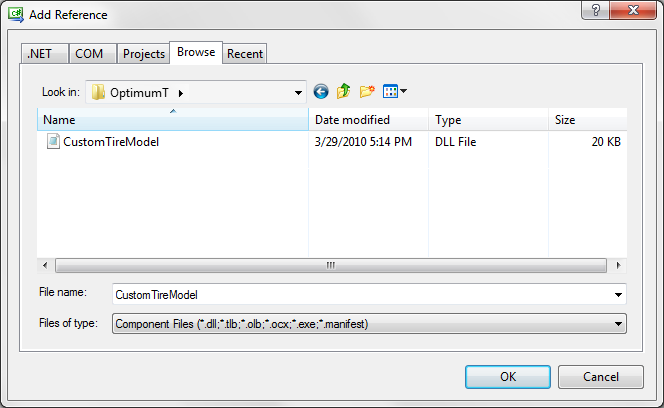
\includegraphics[height=0.4\textheight]{SelectTemplate.png}
	\caption{Selecting the Reference .dll}
	\label{fig:SelectingtheReferencedll}
\end{figure}

\subsection{Creating a Coefficient File}
\label{sec:CreatingaCoefficientFile}

An example coefficient file has been included with the OptimumTire custom package. It is shown in Figure~\ref{fig:CoefFileVC}. It has a number of features. 

 \begin{figure}[H]
	\centering
		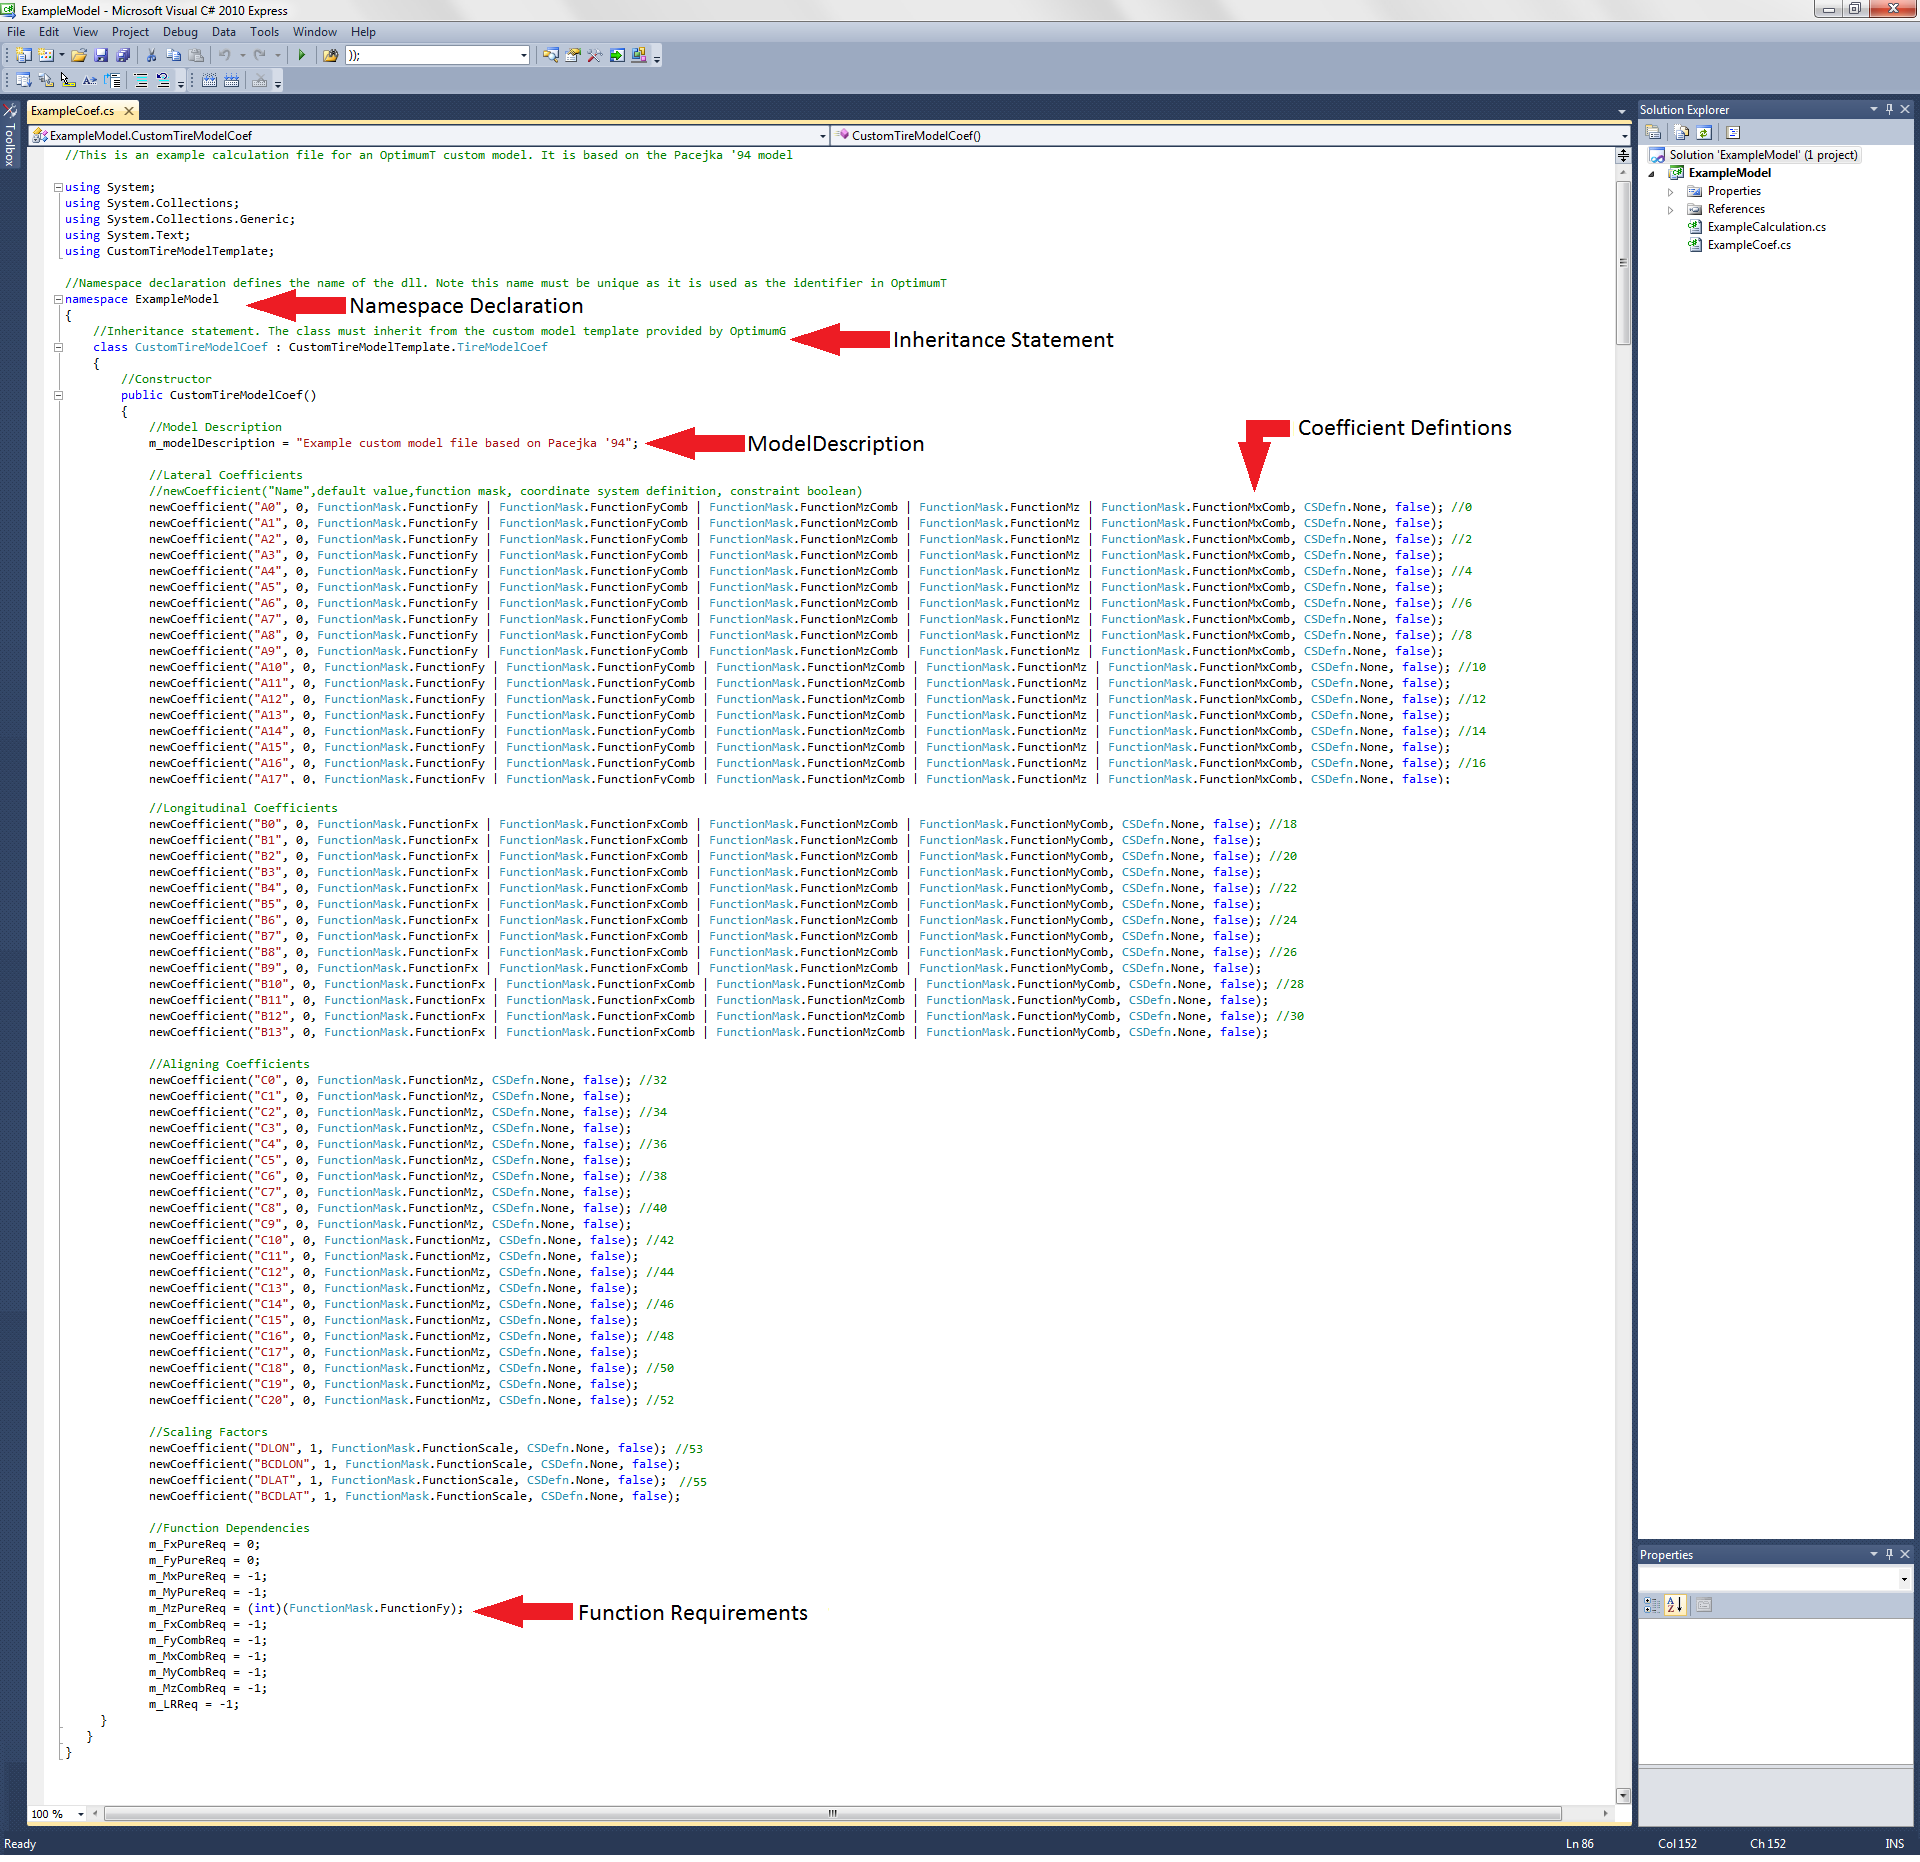
\includegraphics[width=1.0\textwidth]{CoefFileVC.png}
	\caption{Visual C\# Coefficient File}
	\label{fig:CoefFileVC}
\end{figure}

The first section is the \textsl{\textquotedbl Namespace Declaration\textquotedbl} this is the name of the custom .dll file and will be used as an identifier within OptimumTire.

The second statement is the \textsl{\textquotedbl Inheritance Statement\textquotedbl}. This is required to ensure all the template functions are available to the custom .dll. Without this statement the .dll will produce an error when loaded into OptimumTire. The coefficient file must inherit from the coefficient template CustomTireModelTemplate.TireModelCoef.

The third statement is the \textsl{\textquotedbl Model Description\textquotedbl} which will appear in the description box on the model coefficient form sheet.

The fourth section contains the \textsl{\textquotedbl Coefficient Definitions\textquotedbl} themselves. It is a list of the coefficients to be added to the array list. These statements are in the format shown at the start of this section.

The fifth section is the \textsl{\textquotedbl Function Requirements\textquotedbl}. These statements allow the user to change the function dependencies in the model. For example the aligning moment function often requires the the lateral force to be calculated frist. Therefore the function requirement for \textsl{CalculateMz} will be \textsl{FunctionMask.FunctionFy}. The function requirements statements are in the following syntax.

\textbf{\texttt{m\_MzPureReq = (int)(FunctionMask.FunctionFy);}}

setting a function requirement equal to -1 will make that function unavailable. Setting the requirement equal to 0 indicates that the function does not have any dependencies.

The coefficient file is simply an arraylist of coefficients. Each coefficient is defined in the following format:

\texttt{\textbf{newCoefficient((\textquotedbl Name\textquotedbl , Default Value, Function Mask, Coordinate System Definition, Constraint Boolean)}}

\begin{itemize}
\item	\textbf{Name:} The name of the variable that will appear beside each variable in OptimumTire.  Must be entered as a string enclosed in quotation marks \textquotedbl \textquotedbl
\item	\textbf{Default Value:} The default value of the coefficient that will apear when creating empty models, boundary files and constraints. This value is a single floating point number.
\item \textbf{Function Mask:} Tells OptimumTire which outputs are related to each coefficient so the solver knows which coefficients to fit when fitting a specific model. OptimumTire has a list of function masks to choose from:


\begin{center}

\texttt{\textbf{FunctionMask.FunctionFx \\
FunctionMask.FunctionFy \\
FunctionMask.FunctionFz \\
FunctionMask.FunctionMx \\
FunctionMask.FunctionMy \\
FunctionMask.FunctionMz \\
FunctionMask.FunctionRl \\
FunctionMask.FunctionScale}}
\end{center}

Each coefficient must include one of these definition or a combination of the above separated by the or \textquotedbl | \textquotedbl operator. 

For example a coefficient \textsl{\textquotedbl U\textquotedbl} is used in the equations for calculating the lateral force, longitudinal force and aligning torque its coefficient mask is therefore:

\texttt{\textbf{FunctionMask.FunctionFx | FunctionMask.FunctionFy | FunctionMask.FunctionMz}}

The function mask FunctionScale is used to specify that the coefficient is used as a scaling factor(see Section~\ref{sec:ModelScalingFactors}). This means the coefficient will not be fit in the fitting proccess and will remain the default value specified. The default value should be 1.0 in most cases for the scaling factors to have no effect on the model.

\item \textbf{Coordinate System Definition:} The coordinate properties of the coefficient that determine which coordinate system conversion will cause the coefficient to change sign. Each coordinate system definition is in the form CSDfn.X which means, that if the sign of the input X changes in a coordinate system  conversion the coefficients with the corresponding coordinate system definition will also change sign. OptimumTire provides the following coordinate system definitions:
 	
\begin{center}

\texttt{\textbf{   	CSDefn.V \\
    CSDefn.SA \\
    CSDefn.SR \\
    CSDefn.IA \\
    CSDefn.F~\_x \\
    CSDefn.F~\_y \\
    CSDefn.F~\_z \\
    CSDefn.M~\_x \\
    CSDefn.M~\_y \\
    CSDefn.M~\_z \\
    CSDefn.None}}
\end{center}

Note: Leaving the coordinate system definition as \textsl{CSDefn.None} means the coefficient will not be affected by any coordinate system conversions within OptimumTire so the coefficients will always remain in the initially selected system.

OptimumTire supports four coordinate systems these are the SAE, Adapted SAE, ISO and Adapted ISO coordinate systems. For definitions of these systems see Section~\ref{sec:CoordinateSystems}. These coordinate systems will apply the following coordinate system changes when converting from the default SAE coordinate system:

        \textbf{SAE:} {\tt Default} \\
        \textbf{Adapted SAE:}  {\tt CSDefn.SA | CSDefn.F\_z} \\
        \textbf{ISO:} {\tt CSDefn.SA | CSDefn.F\_y | CSDefn.F\_z | CSDefn.M\_y | CSDefn.M\_z} \\
        \textbf{Adapted ISo:} {\tt CSDefn.IA | CSDefn.F\_y | CSDefn.F\_z | CSDefn.M\_y | CSDefn.M\_z}

\item \textbf{Constraint Boolean:} Defines whether a coefficient will be a fixed constraint or not. True if coefficient of fixed or false if it is a coefficient is to be fit.
\end{itemize}

\subsection{Creating a Calculation File}
\label{sec:CreatingaCalculationFile}

The calculation file contains the equations that define the tire model. An example of how to create a calculation file is included with the OptimumTire custom model package. The example is shown in Figure~\ref{fig:CalcFileVC}.

 \begin{figure}[H]
	\centering
		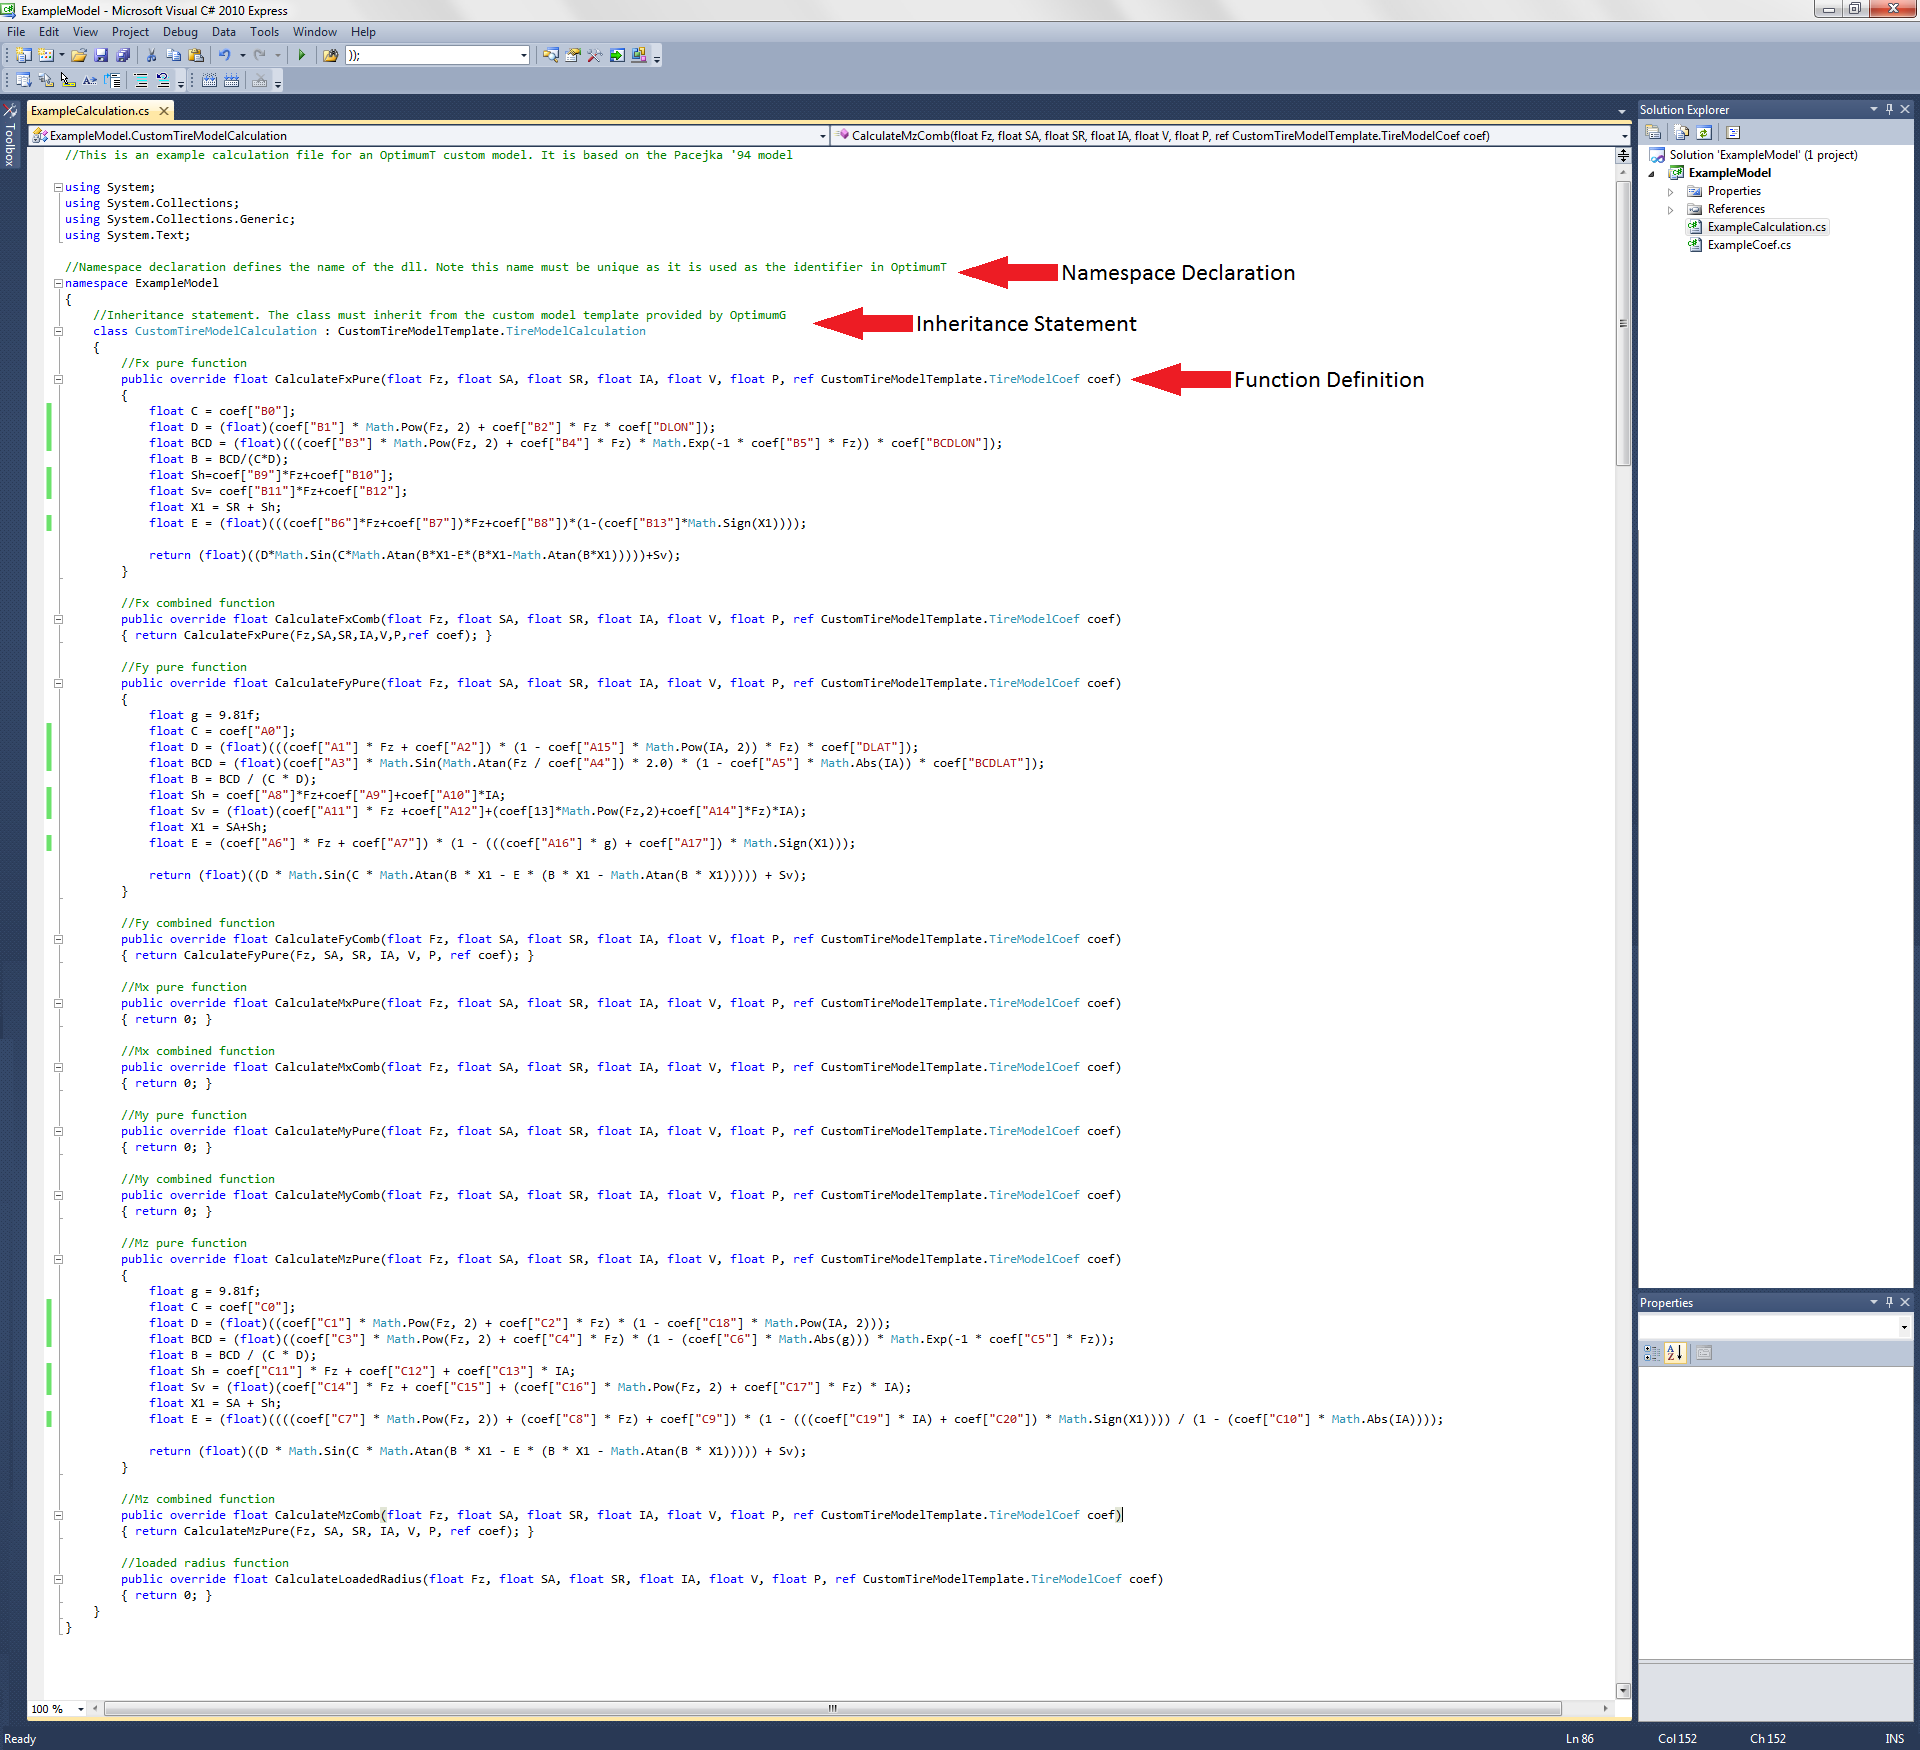
\includegraphics[width=1.0\textwidth]{CalcFileVC.png}
	\caption{Visual C\# Calculation File}
	\label{fig:CalcFileVC}
\end{figure}

The file contains several statements. The first is the \textsl{\textquotedbl Namespace Declaration\textquotedbl} this is the name of the .dll and will be used by OptimumTire as an identifier for the custom model. It must be the same as the \textsl{\textquotedbl Namespace Declaration\textquotedbl} in the coefficient file.

The second statement is the \textsl{\textquotedbl Inheritance Statement\textquotedbl}. This is required to ensure all the template functions are available to the custom .dll. Without this statement the .dll will produce an error when loaded into OptimumTire. The coefficient file must inherit from the calculation template CustomTireModelTemplate.TireModelCalculation.

The third section contains the function definitons themselves. The primary functions must be declared in the following format to override the fucntions in the template file.

\texttt{\textbf{public override float CalculateXXXXX(float Fz, float SA, float SR, float IA, float V, float P, ref CustomTireModelTemplate.TireModelCoef coef)}}

The custom calculation template contains the following overridable functions that can be redefined by the user.

\begin{center}
\texttt{\textbf{CalculateFxPure(Fz, SA, SR, IA, V, P, ref coef)\\
	        CalculateFxComb(Fz, SA, SR, IA, V, P, ref coef)\\
	        CalculateFyPure(Fz, SA, SR, IA, V, P, ref coef)\\
	        CalculateFyComb(Fz, SA, SR, IA, V, P, ref coef)\\
	        CalculateMxPure(Fz, SA, SR, IA, V, P, ref coef)\\
	        CalculateMxComb(Fz, SA, SR, IA, V, P, ref coef)\\
	        CalculateMyPure(Fz, SA, SR, IA, V, P, ref coef)\\
	        CalculateMyComb(Fz, SA, SR, IA, V, P, ref coef)\\
	        CalculateMzPure(Fz, SA, SR, IA, V, P, ref coef)\\
	        CalculateMzComb(Fz, SA, SR, IA, V, P, ref coef)\\
	        CalculateLoadedRadius(Fz, SA, SR, IA, V, P, ref coef)}}
\end{center}

    
These functions define the primary outputs of OptimumTire. The user may include any number of additional functions that may be called from within these primary functions. It should be noted that the quality of the code in the calculation file will affect the speed of the fitting and graphing processes.
Each function must follow the signature of the functions defined in the template file. Each function returns a single floating point value for the input values Fz, SA, SR, IA, V, P and the coefficient array.

When writing the functions themselves the user can refer to the coefficients by their name as previously defined in the coefficient file. eg. {\tt coef[\textquotedbl A0 \textquotedbl]}. 

\subsection{Common Programming Errors}
\label{sec:Common Programming Errors}
The following are common errors made when programming in C\#. Check the following basic syntax before compiling your custom .dll.

\begin{itemize}
	\item In C\# each command should be placed on a new line which ends with the \textquotedbl ;\textquotedbl character.

\item Functions, classes, loops and conditional statements are defined by braces. Each \textquotedbl \{\textquotedbl must have a matching  \textquotedbl \}\textquotedbl.

\item Each function must have the correct signature. Use intellisense to make sure that each function passes all the required parameters.
\end{itemize}

For more information on programming in C\# see ~\href{http://www.msdn.com}{www.msdn.com}

\section{Importing Custom Models in OptimumTire}
\label{sec:ImportingCustomModelsinOptimumTire}

Once the user has created or been given a custom model .dll file it can be loaded into OptimumTire. To load the custom model select the \textsl{Advanced} menu item in OptimumTire then selct the \textsl{Custom Tire Model} item from the dropdown menu as shown in Figure~\ref{fig:AdvancedFeaturesMenu}.

\begin{figure}[H]
	\centering
		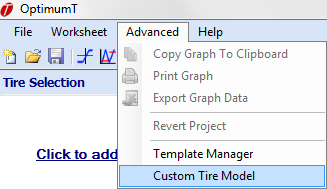
\includegraphics{AdvancedCustomTireModel.png}
	\caption{Advanced Features Menu}
	\label{fig:AdvancedFeaturesMenu}
\end{figure}

Selecting the \textsl{Custom Tire Model} item will launch the \textsl{Custom Tire Model Manager} shown in Figure~\ref{fig:CustomTireModelManager}.

 \begin{figure}[H]
	\centering
		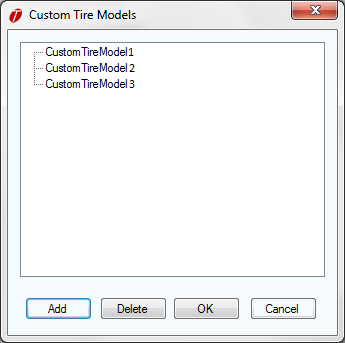
\includegraphics{CustomTireModelManager.png}
	\caption{Custom Tire Model Manager}
	\label{fig:CustomTireModelManager}
\end{figure}

The \textsl{Custom Tire Model Manager} shows the list of custom models currently available in OptimumTire. The user can add or delete models from the list using the add and delete buttons. Note that OptimumTire uses the name of the .dll as an identifier so two custom models cannot be added with the same name. See sections~\ref{sec:CreatingaCoefficientFile} and ~\ref{sec:CreatingaCalculationFile} for how to name custom models.

Clicking on the \textsl{Add} button opens a standard windows dialog. Navigate to the location of the custom .dll that is to be added and click \textsl{OK} to add the model to the list.

\section{The Custom Model Fitting Process}
\label{sec:The CustomModelFittingProcess}

To fit a custom model the user can follow the same process used for standard model fitting. The \textsl{Custom Model} option should appear at the bottom of the list of models available to fit in the model fitting dropdown menu as shown in Figure~\ref{fig:CustomModelFitting}.

 \begin{figure}[H]
	\centering
		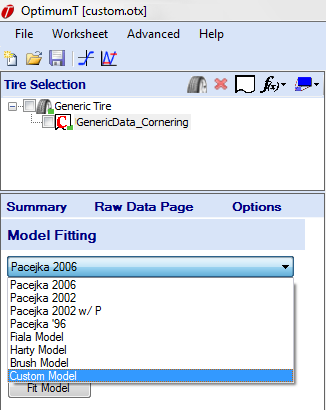
\includegraphics{CustomFitting.png}
	\caption{Custom Model Fitting}
	\label{fig:CustomModelFitting}
\end{figure}

Selecting the \textsl{Custom Model} item from the dropdown will bring up the \textsl{Custom Model Selection Dialog} shown in Figure~\ref{fig:CustomTireModelSelection}. Select the custom model to be fit by either double clicking on it, or selecting it and clicking the \textsl{OK} button. This will launch the fitting process.

The main differences in the custom fitting process are the constraints and boundary files. Which coefficients appear in the \textsl{Constraints Wizard} will depend on the \textsl{Constraint Boolean} specified in the coefficient file created by the user (see Section~\ref{sec:CreatingaCoefficientFile}). Also the boundaries wizard will not contain predefined templates so a new boundary must be created for each new custom model.

 \begin{figure}[H]
	\centering
		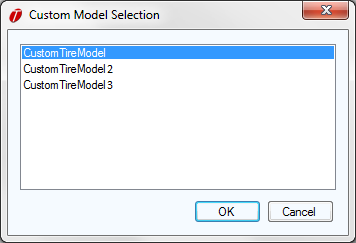
\includegraphics{CustomModelSelection.png}
	\caption{Custom Tire Model Selection}
	\label{fig:CustomTireModelSelection}
\end{figure}

\section{Custom Model Import and Export}
\label{sec:CustomModelImportandExport}

The import and export functions work for the custom model in the same way as the standard tire models in OptimumTire (see Section~\ref{sec:ImportandExportModels}).

However to export models to .tir or Excel format the user must first create a template for each model. The process for creating and modifying export templates is illustrated in Section~\ref{sec:ImportandExportModelsExportTemplate}.